% Options for packages loaded elsewhere
\PassOptionsToPackage{unicode}{hyperref}
\PassOptionsToPackage{hyphens}{url}
%
\documentclass[
]{book}
\usepackage{amsmath,amssymb}
\usepackage{lmodern}
\usepackage{iftex}
\ifPDFTeX
  \usepackage[T1]{fontenc}
  \usepackage[utf8]{inputenc}
  \usepackage{textcomp} % provide euro and other symbols
\else % if luatex or xetex
  \usepackage{unicode-math}
  \defaultfontfeatures{Scale=MatchLowercase}
  \defaultfontfeatures[\rmfamily]{Ligatures=TeX,Scale=1}
\fi
% Use upquote if available, for straight quotes in verbatim environments
\IfFileExists{upquote.sty}{\usepackage{upquote}}{}
\IfFileExists{microtype.sty}{% use microtype if available
  \usepackage[]{microtype}
  \UseMicrotypeSet[protrusion]{basicmath} % disable protrusion for tt fonts
}{}
\makeatletter
\@ifundefined{KOMAClassName}{% if non-KOMA class
  \IfFileExists{parskip.sty}{%
    \usepackage{parskip}
  }{% else
    \setlength{\parindent}{0pt}
    \setlength{\parskip}{6pt plus 2pt minus 1pt}}
}{% if KOMA class
  \KOMAoptions{parskip=half}}
\makeatother
\usepackage{xcolor}
\usepackage{color}
\usepackage{fancyvrb}
\newcommand{\VerbBar}{|}
\newcommand{\VERB}{\Verb[commandchars=\\\{\}]}
\DefineVerbatimEnvironment{Highlighting}{Verbatim}{commandchars=\\\{\}}
% Add ',fontsize=\small' for more characters per line
\usepackage{framed}
\definecolor{shadecolor}{RGB}{248,248,248}
\newenvironment{Shaded}{\begin{snugshade}}{\end{snugshade}}
\newcommand{\AlertTok}[1]{\textcolor[rgb]{0.94,0.16,0.16}{#1}}
\newcommand{\AnnotationTok}[1]{\textcolor[rgb]{0.56,0.35,0.01}{\textbf{\textit{#1}}}}
\newcommand{\AttributeTok}[1]{\textcolor[rgb]{0.77,0.63,0.00}{#1}}
\newcommand{\BaseNTok}[1]{\textcolor[rgb]{0.00,0.00,0.81}{#1}}
\newcommand{\BuiltInTok}[1]{#1}
\newcommand{\CharTok}[1]{\textcolor[rgb]{0.31,0.60,0.02}{#1}}
\newcommand{\CommentTok}[1]{\textcolor[rgb]{0.56,0.35,0.01}{\textit{#1}}}
\newcommand{\CommentVarTok}[1]{\textcolor[rgb]{0.56,0.35,0.01}{\textbf{\textit{#1}}}}
\newcommand{\ConstantTok}[1]{\textcolor[rgb]{0.00,0.00,0.00}{#1}}
\newcommand{\ControlFlowTok}[1]{\textcolor[rgb]{0.13,0.29,0.53}{\textbf{#1}}}
\newcommand{\DataTypeTok}[1]{\textcolor[rgb]{0.13,0.29,0.53}{#1}}
\newcommand{\DecValTok}[1]{\textcolor[rgb]{0.00,0.00,0.81}{#1}}
\newcommand{\DocumentationTok}[1]{\textcolor[rgb]{0.56,0.35,0.01}{\textbf{\textit{#1}}}}
\newcommand{\ErrorTok}[1]{\textcolor[rgb]{0.64,0.00,0.00}{\textbf{#1}}}
\newcommand{\ExtensionTok}[1]{#1}
\newcommand{\FloatTok}[1]{\textcolor[rgb]{0.00,0.00,0.81}{#1}}
\newcommand{\FunctionTok}[1]{\textcolor[rgb]{0.00,0.00,0.00}{#1}}
\newcommand{\ImportTok}[1]{#1}
\newcommand{\InformationTok}[1]{\textcolor[rgb]{0.56,0.35,0.01}{\textbf{\textit{#1}}}}
\newcommand{\KeywordTok}[1]{\textcolor[rgb]{0.13,0.29,0.53}{\textbf{#1}}}
\newcommand{\NormalTok}[1]{#1}
\newcommand{\OperatorTok}[1]{\textcolor[rgb]{0.81,0.36,0.00}{\textbf{#1}}}
\newcommand{\OtherTok}[1]{\textcolor[rgb]{0.56,0.35,0.01}{#1}}
\newcommand{\PreprocessorTok}[1]{\textcolor[rgb]{0.56,0.35,0.01}{\textit{#1}}}
\newcommand{\RegionMarkerTok}[1]{#1}
\newcommand{\SpecialCharTok}[1]{\textcolor[rgb]{0.00,0.00,0.00}{#1}}
\newcommand{\SpecialStringTok}[1]{\textcolor[rgb]{0.31,0.60,0.02}{#1}}
\newcommand{\StringTok}[1]{\textcolor[rgb]{0.31,0.60,0.02}{#1}}
\newcommand{\VariableTok}[1]{\textcolor[rgb]{0.00,0.00,0.00}{#1}}
\newcommand{\VerbatimStringTok}[1]{\textcolor[rgb]{0.31,0.60,0.02}{#1}}
\newcommand{\WarningTok}[1]{\textcolor[rgb]{0.56,0.35,0.01}{\textbf{\textit{#1}}}}
\usepackage{longtable,booktabs,array}
\usepackage{calc} % for calculating minipage widths
% Correct order of tables after \paragraph or \subparagraph
\usepackage{etoolbox}
\makeatletter
\patchcmd\longtable{\par}{\if@noskipsec\mbox{}\fi\par}{}{}
\makeatother
% Allow footnotes in longtable head/foot
\IfFileExists{footnotehyper.sty}{\usepackage{footnotehyper}}{\usepackage{footnote}}
\makesavenoteenv{longtable}
\usepackage{graphicx}
\makeatletter
\def\maxwidth{\ifdim\Gin@nat@width>\linewidth\linewidth\else\Gin@nat@width\fi}
\def\maxheight{\ifdim\Gin@nat@height>\textheight\textheight\else\Gin@nat@height\fi}
\makeatother
% Scale images if necessary, so that they will not overflow the page
% margins by default, and it is still possible to overwrite the defaults
% using explicit options in \includegraphics[width, height, ...]{}
\setkeys{Gin}{width=\maxwidth,height=\maxheight,keepaspectratio}
% Set default figure placement to htbp
\makeatletter
\def\fps@figure{htbp}
\makeatother
\setlength{\emergencystretch}{3em} % prevent overfull lines
\providecommand{\tightlist}{%
  \setlength{\itemsep}{0pt}\setlength{\parskip}{0pt}}
\setcounter{secnumdepth}{5}
\usepackage{booktabs}
\ifLuaTeX
  \usepackage{selnolig}  % disable illegal ligatures
\fi
\usepackage[]{natbib}
\bibliographystyle{plainnat}
\IfFileExists{bookmark.sty}{\usepackage{bookmark}}{\usepackage{hyperref}}
\IfFileExists{xurl.sty}{\usepackage{xurl}}{} % add URL line breaks if available
\urlstyle{same} % disable monospaced font for URLs
\hypersetup{
  pdftitle={Welcome to my portofolio},
  pdfauthor={Lamyae el Mahboud},
  hidelinks,
  pdfcreator={LaTeX via pandoc}}

\title{Welcome to my portofolio}
\author{Lamyae el Mahboud}
\date{2023-05-15}

\begin{document}
\maketitle

{
\setcounter{tocdepth}{1}
\tableofcontents
}
\hypertarget{my-portofolio}{%
\chapter{My portofolio}\label{my-portofolio}}

\hypertarget{introduction}{%
\section{introduction}\label{introduction}}

Welcome to my portofolio. My name is Lamyae and im studying at the Utrecht University of Applied Sciences.

In this github page you'll find different skills.

\hypertarget{c.-elegans-plate-experiment-analysis}{%
\chapter{C. elegans plate experiment analysis}\label{c.-elegans-plate-experiment-analysis}}

\hypertarget{introduction-1}{%
\section{Introduction}\label{introduction-1}}

In this exercise we will read and analyze a data file. While analyzing the data we come across a few issues we try to fix. The data we're gonna use in this exercise was derived from an experiment in which adult C.elegans were exposed to varying concentrations of different compounds. The variables RawData (the outcome - number of offspring counted as an integer value, after incubation time), compName (the generic name of the compound/chemical), the compConcentration (the concentration of the compound), and the expType are the most important variables in this dataset.

After we reviewed the Excel File. We see in the Excel file that there is no data in the colomns `plateRow' en `plateColmn'.
Some colomns arent nesecerasy like `expDate', `expResearcher', `expTime', `éxpUnit'. This kind of information is metadata and should not be in your rawdata. It makes the table cluttered and information less easy to find.
Some data in colomn is the same for all coditions, like `compDelivery' and `bacterialStrain'. This kind of information is metadata and shouldn't be in your table.

after reviewing the file we want to open the excel file in R using the \{readxl\} package.

\begin{Shaded}
\begin{Highlighting}[]
\FunctionTok{library}\NormalTok{(tidyverse) }\CommentTok{\#load in tidyverse package}
\FunctionTok{library}\NormalTok{(readxl) }\CommentTok{\#load in readxl package }

\NormalTok{data }\OtherTok{\textless{}{-}} \FunctionTok{read\_excel}\NormalTok{(}\StringTok{"CE.LIQ.FLOW.062\_Tidydata.xlsx"}\NormalTok{) }\CommentTok{\#load in the data that we want to use for this assignment}
\end{Highlighting}
\end{Shaded}

Before we go ahead an start analyzing our data. We're gonna inspect the following colomns: ``Rawdata'', ``compName'' and ``compConcentration''

\begin{Shaded}
\begin{Highlighting}[]
\FunctionTok{head}\NormalTok{(data[}\FunctionTok{c}\NormalTok{(}\StringTok{\textquotesingle{}RawData\textquotesingle{}}\NormalTok{, }\StringTok{\textquotesingle{}compName\textquotesingle{}}\NormalTok{, }\StringTok{\textquotesingle{}compConcentration\textquotesingle{}}\NormalTok{)]) }\CommentTok{\#we want to see the first few lines of the colomns RawData compName and compConcentration}
\end{Highlighting}
\end{Shaded}

\begin{verbatim}
## # A tibble: 6 x 3
##   RawData compName                   compConcentration
##     <dbl> <chr>                      <chr>            
## 1      44 2,6-diisopropylnaphthalene 4.99             
## 2      37 2,6-diisopropylnaphthalene 4.99             
## 3      45 2,6-diisopropylnaphthalene 4.99             
## 4      47 2,6-diisopropylnaphthalene 4.99             
## 5      41 2,6-diisopropylnaphthalene 4.99             
## 6      35 2,6-diisopropylnaphthalene 4.99
\end{verbatim}

The colomn `Rawdata' is a ``dbl'' type, this is what we expected.
The colomn `compName' is a ``chr'' type, this is what we expected .
The colomn `compConcentration' is a ``chr'' type, this is not correct since they are only numbers in the colomn.

We're gonna make a scatterplot for the data. As you can see in the code below we put the ``compConcentration'' on the x-axis, the ``Rawdata'' counts on the y-axis. For each level in ``compName'' we assign a colour and for each level in ``expType'' we assign a different symbol.

\begin{Shaded}
\begin{Highlighting}[]
\FunctionTok{library}\NormalTok{(tidyverse) }\CommentTok{\#load in the tidyverse data}

\FunctionTok{ggplot}\NormalTok{(}\AttributeTok{data =}\NormalTok{ data, }\FunctionTok{aes}\NormalTok{(}\AttributeTok{x =}\NormalTok{ compConcentration, }\AttributeTok{y =}\NormalTok{ RawData )) }\SpecialCharTok{+}
  \FunctionTok{geom\_point}\NormalTok{(}\FunctionTok{aes}\NormalTok{(}\AttributeTok{color =}\NormalTok{ compName, }
                 \AttributeTok{shape =}\NormalTok{ expType)) }\CommentTok{\#scatterplot for the different compounds and the varying concentrations}
\end{Highlighting}
\end{Shaded}

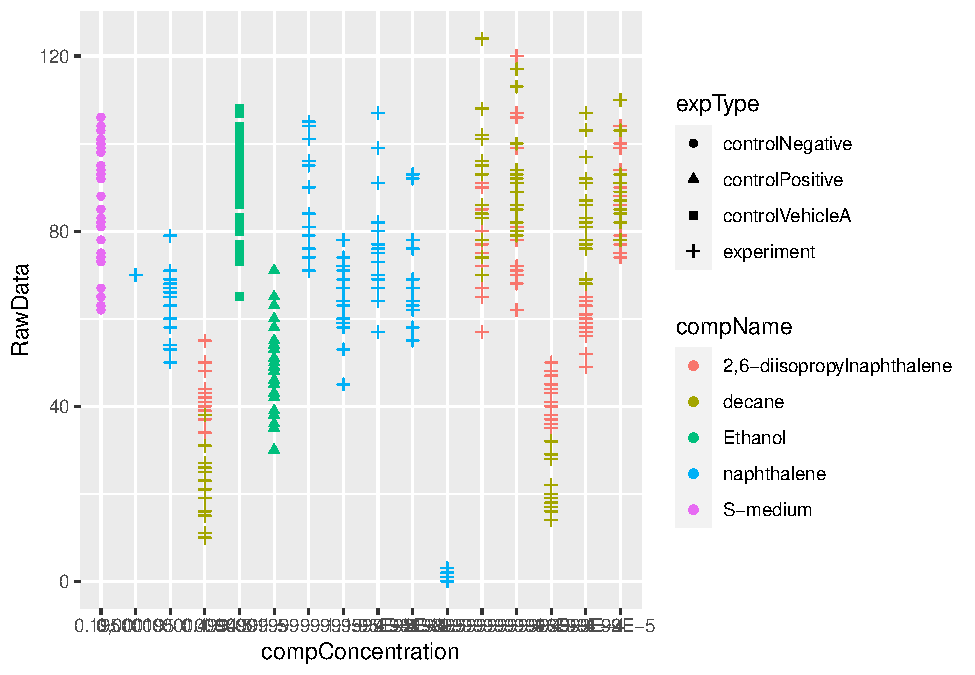
\includegraphics{_main_files/figure-latex/wrongplot-1.pdf}

We just made a scatterplot with the data from the excel file we imported earlier. Each compName has its own colour and each expType has its own shape, but we see one big problem. As we can see is the x-axis not very readable, actually not at all!

when we imported the Excel file, the colomn `compConcentration' had a charachter type. Because of this every single charachter in each cell was shown on the x-axis and the numbers weren't rounded. This explains why the x-axis wasn't readable.

To correct this mistake, we're gonna change the type of the colomn ``compConcentration'' from ``chr'' to ``dbl''.

\begin{Shaded}
\begin{Highlighting}[]
\NormalTok{data}\SpecialCharTok{$}\NormalTok{compConcentration }\OtherTok{\textless{}{-}} \FunctionTok{as.numeric}\NormalTok{(data}\SpecialCharTok{$}\NormalTok{compConcentration) }\CommentTok{\#change the type of the colomn from \textless{}chr\textgreater{} to \textless{}dbl\textgreater{}}

\FunctionTok{library}\NormalTok{(tidyverse) }\CommentTok{\#load in tidyverse package}

\FunctionTok{ggplot}\NormalTok{(}\AttributeTok{data =}\NormalTok{ data, }\FunctionTok{aes}\NormalTok{(}\AttributeTok{x =} \FunctionTok{log10}\NormalTok{(compConcentration), }\AttributeTok{y =}\NormalTok{ RawData)) }\SpecialCharTok{+}
  \FunctionTok{geom\_jitter}\NormalTok{(}\FunctionTok{aes}\NormalTok{(}\AttributeTok{color =}\NormalTok{ compName, }
                 \AttributeTok{shape =}\NormalTok{ expType),}
             \AttributeTok{size =} \DecValTok{3}\NormalTok{,}\AttributeTok{alpha =} \FloatTok{0.8}\NormalTok{) }\SpecialCharTok{+}
  \FunctionTok{labs}\NormalTok{(}\AttributeTok{title =} \StringTok{"Rawdata of each compName and their expType"}\NormalTok{,}
       \AttributeTok{y =} \StringTok{"Rawdata"}\NormalTok{,}
       \AttributeTok{x =} \StringTok{"compConcentration(nM)"}\NormalTok{) }\SpecialCharTok{+}
  \FunctionTok{theme\_minimal}\NormalTok{() }\CommentTok{\#scatterplot of the data with fixed x{-}axis and jitter}
\end{Highlighting}
\end{Shaded}

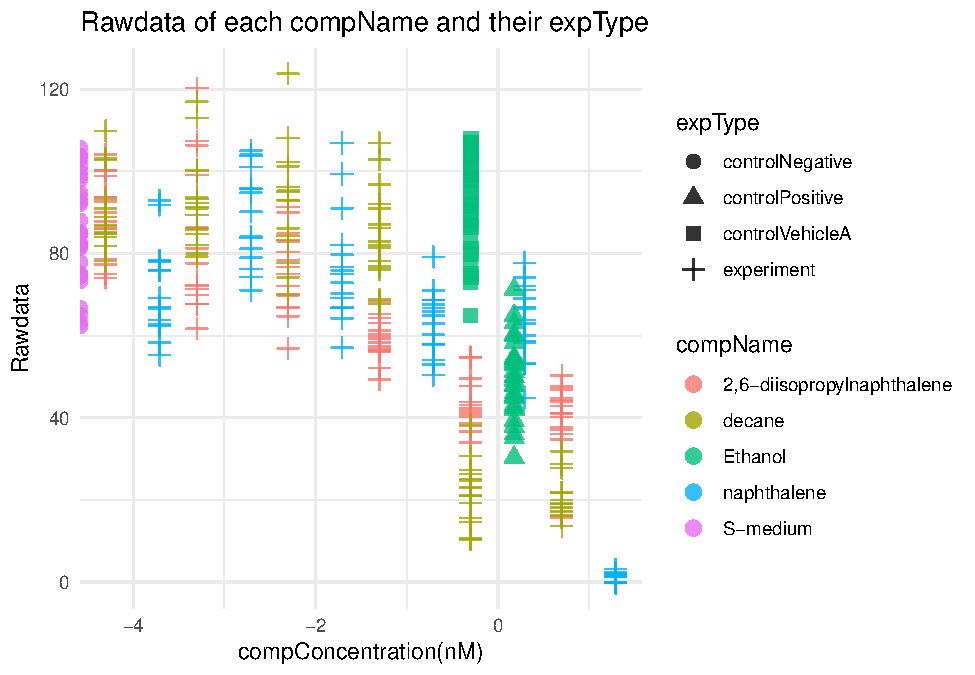
\includegraphics{_main_files/figure-latex/fixingplot-1.pdf}

As we van see the x-axis is now readable.

We see in the scatterplot that the positive control for this experiments is Ethanol. The negative control for this experiment is S-medium.

if we really want to compare the different between the compund and experiments type. We need to normalize the data for the Negative control. We normalize the data by setting the mean value for the ``controlNegative'' to 1. All the other values are expressed as a fraction thereof.

\begin{Shaded}
\begin{Highlighting}[]
\FunctionTok{library}\NormalTok{(tidyverse)}

\NormalTok{data\_df }\OtherTok{\textless{}{-}} \FunctionTok{as.data.frame}\NormalTok{(data)}

\NormalTok{controlnegative\_mean }\OtherTok{\textless{}{-}} \FunctionTok{mean}\NormalTok{(data\_df}\SpecialCharTok{$}\NormalTok{RawData[data\_df}\SpecialCharTok{$}\NormalTok{compVehicle }\SpecialCharTok{==} \StringTok{"controlNegative"}\NormalTok{]) }\CommentTok{\#calculate mean of the control negative}

\NormalTok{data\_df}\SpecialCharTok{$}\NormalTok{data\_norm }\OtherTok{\textless{}{-}}\NormalTok{ data\_df}\SpecialCharTok{$}\NormalTok{RawData}\SpecialCharTok{/}\NormalTok{controlnegative\_mean}
  
\FunctionTok{ggplot}\NormalTok{(}\AttributeTok{data =}\NormalTok{ data\_df, }\FunctionTok{aes}\NormalTok{(}\AttributeTok{x =} \FunctionTok{log10}\NormalTok{(compConcentration), }\AttributeTok{y =}\NormalTok{ data\_norm)) }\SpecialCharTok{+}
  \FunctionTok{geom\_jitter}\NormalTok{(}\FunctionTok{aes}\NormalTok{(}\AttributeTok{color =}\NormalTok{ compName, }
                 \AttributeTok{shape =}\NormalTok{ expType),}
             \AttributeTok{size =} \FloatTok{1.5}\NormalTok{,}\AttributeTok{alpha =} \FloatTok{0.8}\NormalTok{, }\AttributeTok{width =} \FloatTok{0.2}\NormalTok{) }\SpecialCharTok{+}
  \FunctionTok{labs}\NormalTok{(}\AttributeTok{title =} \StringTok{"Rawdata of each compName and their expType"}\NormalTok{,}
       \AttributeTok{y =} \StringTok{"Rawdata normalized"}\NormalTok{,}
       \AttributeTok{x =} \StringTok{"compConcentration(nM)"}\NormalTok{) }\SpecialCharTok{+}
  \FunctionTok{theme\_minimal}\NormalTok{() }\CommentTok{\#scatterplot of the data with fixed x{-}axis and jitter}
\end{Highlighting}
\end{Shaded}

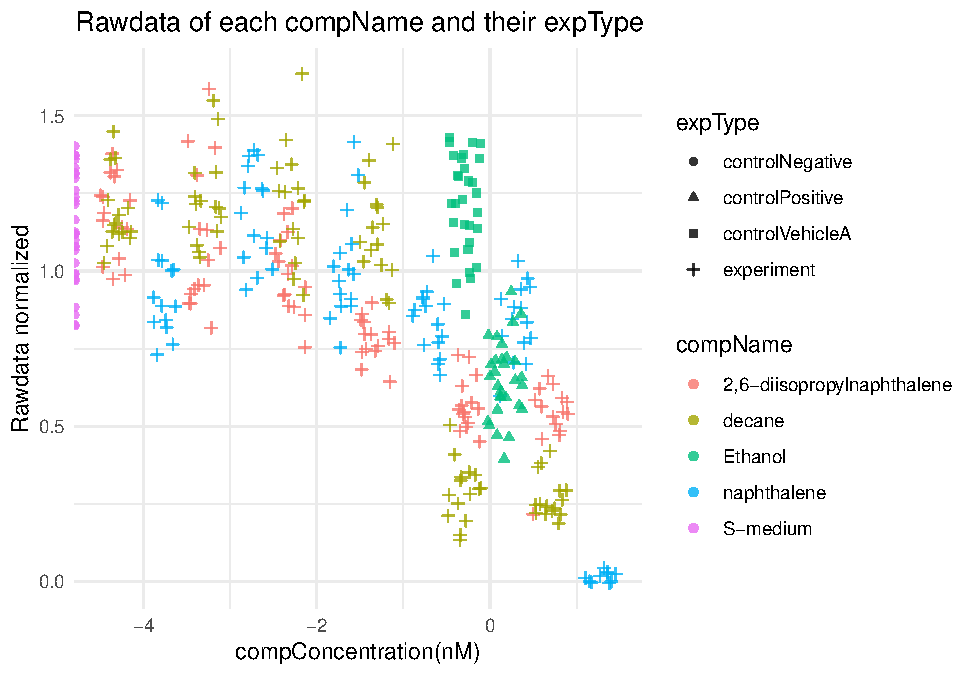
\includegraphics{_main_files/figure-latex/fixedplot-1.pdf}

In the dataset we used for this analysis, each compound has his own concentrations. If we want make the data more comparable we have to normalize the data.

\hypertarget{analyzing-plan}{%
\section{analyzing plan}\label{analyzing-plan}}

If we want to analyze the data to learn whether there is indeed an effect of different concentrations on offspring count and whether the different compounds have a different curve(ic50), First we need to get the data and prepare it. We did this already as you can see above.

after preparing the data we will perform the shapiro.test for every compound to check if the data (Rawdata) is normally distributed. All compounds need to have a p-value greater than 0.05.

To test if there is a significant difference between compound concentrations we can use the one sample t-test for each compound individually. To do this we have to filter the table for the compound we want to test first before we perform the test.

To compare the IC50 of each compound we can use the
\{drc\} package to visualize the different curves for each compound.

\hypertarget{open-peer-review}{%
\chapter{Open Peer Review}\label{open-peer-review}}

\hypertarget{introduction-2}{%
\section{Introduction}\label{introduction-2}}

We're gonna identify reproducibility issues in a scientific publication. We use the \href{https://www.researchgate.net/publication/340244621_Reproducibility_and_reporting_practices_in_COVID-19_preprint_manuscripts}{criteria for reproduciblity} to see if our article is reproducible or not. The scientific article that we use can be found \href{https://www.ncbi.nlm.nih.gov/pmc/articles/PMC4173157/}{here}.

\begin{table}

\caption{\label{tab:unnamed-chunk-5}Table1: The Transparency Criteria scores of the scientific article}
\centering
\begin{tabular}[t]{l|l}
\hline
transparency Criteria & Available\\
\hline
Study Purpose & Yes\\
\hline
Data Availability Statement & No\\
\hline
Data Location & No\\
\hline
Study Location & No\\
\hline
Author Review & Yes\\
\hline
Ethics Statement & No\\
\hline
Funcing statement & Yes\\
\hline
Code Availability & No\\
\hline
\end{tabular}
\end{table}

\hypertarget{clarification}{%
\section{Clarification}\label{clarification}}

We've read the article and scored the article based on the Transparency Criteria in table 1. For each ``Yes'' in ``Availability'' the article scores one point. As we can see in table 1 the article scores four points out of eight. This article is not reproducible.

The authors give us a statement why they started this research in the last paragraph.
Although they show all their results, there is no raw data available of the western blot or the qPCR.

The data of this study cant be accessed. There is no file or link with the raw or processed data available, only results.

The paper doesn't provide the exact study location in the methods section or else where. However it does give us a few laboratories where the research is done, like the Jackson Laboratory and the Bartek Laboratory. But since these laboratories have multiple locations we still don't know where they performed the experiments.

In the paper is an e-mail adress of one of the authors. There are no contact information of the other authors.
The paper doesn't give us a statement within the paper indicating any ethical concerns.
The paper does give us a statement within the paper indicating that the authors received funding for their research. In the last paragraph under Results and Discussion the authors give use a summary of all their findings.

The codes that the researchers used in this experiment are not available for the reader.

\hypertarget{the-second-peer-review}{%
\section{the second peer review}\label{the-second-peer-review}}

h and i.
\url{https://osf.io/87mpk}

\begin{enumerate}
\def\labelenumi{\alph{enumi}.}
\setcounter{enumi}{9}
\item
  This code is analyzing two countries, the USA and India.
\item
  This codes scores a two out of five on readability. the codes contain a `header', but it could be more informative. A header like ``Donation'' doesn't give the reader enough information.
\item
  before we could run the code, we hade to download a dataset named ``data.clean.txt''.
\end{enumerate}

\begin{Shaded}
\begin{Highlighting}[]
\FunctionTok{library}\NormalTok{(rethinking)}

\NormalTok{d}\OtherTok{\textless{}{-}}\FunctionTok{read.table}\NormalTok{(}\StringTok{"data.clean.txt"}\NormalTok{,}\AttributeTok{sep=}\StringTok{"}\SpecialCharTok{\textbackslash{}t}\StringTok{"}\NormalTok{,}\AttributeTok{header=}\NormalTok{T,}\AttributeTok{stringsAsFactors =}\NormalTok{ F)}
\FunctionTok{names}\NormalTok{(d)}

\NormalTok{dat }\OtherTok{\textless{}{-}} \FunctionTok{list}\NormalTok{(}
  \AttributeTok{C=}\NormalTok{d}\SpecialCharTok{$}\NormalTok{CountC,}

  \AttributeTok{A =} \FunctionTok{standardize}\NormalTok{(d}\SpecialCharTok{$}\NormalTok{Age),}
  \AttributeTok{G =} \FunctionTok{as.integer}\NormalTok{(}\FunctionTok{as.factor}\NormalTok{(d}\SpecialCharTok{$}\NormalTok{Gender)),  }\CommentTok{\#1 Man, 2 Woman}
  \AttributeTok{CD =} \FunctionTok{as.integer}\NormalTok{(d}\SpecialCharTok{$}\NormalTok{COND),}
  \AttributeTok{Mfm =} \FunctionTok{standardize}\NormalTok{(d}\SpecialCharTok{$}\NormalTok{MAC.fam),}
  \AttributeTok{Mg =} \FunctionTok{standardize}\NormalTok{(d}\SpecialCharTok{$}\NormalTok{MAC.gro),}
  \AttributeTok{Mr =} \FunctionTok{standardize}\NormalTok{(d}\SpecialCharTok{$}\NormalTok{MAC.rec),}
  \AttributeTok{Mh =} \FunctionTok{standardize}\NormalTok{(d}\SpecialCharTok{$}\NormalTok{MAC.her),}
  \AttributeTok{Md =} \FunctionTok{standardize}\NormalTok{(d}\SpecialCharTok{$}\NormalTok{MAC.def),}
  \AttributeTok{Mfi =} \FunctionTok{standardize}\NormalTok{(d}\SpecialCharTok{$}\NormalTok{MAC.fai),}
  \AttributeTok{Mp =} \FunctionTok{standardize}\NormalTok{(d}\SpecialCharTok{$}\NormalTok{MAC.pro),}
  \AttributeTok{P =} \FunctionTok{standardize}\NormalTok{(d}\SpecialCharTok{$}\NormalTok{Precaution),}
  \AttributeTok{S =} \FunctionTok{standardize}\NormalTok{(d}\SpecialCharTok{$}\NormalTok{Prosociality),}
  \AttributeTok{D =} \FunctionTok{standardize}\NormalTok{(d}\SpecialCharTok{$}\NormalTok{donation),}
  
  \AttributeTok{Dgr=}\FunctionTok{standardize}\NormalTok{(d}\SpecialCharTok{$}\NormalTok{danger.for.participant),}
  
  \AttributeTok{CC =} \FunctionTok{ifelse}\NormalTok{(d}\SpecialCharTok{$}\NormalTok{COND}\SpecialCharTok{==}\DecValTok{1}\NormalTok{,}\DecValTok{0}\NormalTok{,}\FunctionTok{ifelse}\NormalTok{(d}\SpecialCharTok{$}\NormalTok{COND}\SpecialCharTok{==}\DecValTok{2}\NormalTok{,}\DecValTok{0}\NormalTok{,}\FunctionTok{ifelse}\NormalTok{(d}\SpecialCharTok{$}\NormalTok{COND}\SpecialCharTok{==}\DecValTok{3}\NormalTok{,}\DecValTok{0}\NormalTok{,}\FunctionTok{ifelse}\NormalTok{(d}\SpecialCharTok{$}\NormalTok{COND}\SpecialCharTok{==}\DecValTok{4}\NormalTok{,}\FunctionTok{standardize}\NormalTok{(d}\SpecialCharTok{$}\NormalTok{MAC.fam),}\FunctionTok{ifelse}\NormalTok{(d}\SpecialCharTok{$}\NormalTok{COND}\SpecialCharTok{==}\DecValTok{5}\NormalTok{,}\FunctionTok{standardize}\NormalTok{(d}\SpecialCharTok{$}\NormalTok{MAC.gro),}\FunctionTok{ifelse}\NormalTok{(d}\SpecialCharTok{$}\NormalTok{COND}\SpecialCharTok{==}\DecValTok{6}\NormalTok{,}\FunctionTok{standardize}\NormalTok{(d}\SpecialCharTok{$}\NormalTok{MAC.rec),}\FunctionTok{ifelse}\NormalTok{(d}\SpecialCharTok{$}\NormalTok{COND}\SpecialCharTok{==}\DecValTok{7}\NormalTok{,}\FunctionTok{standardize}\NormalTok{(d}\SpecialCharTok{$}\NormalTok{MAC.her),}\FunctionTok{ifelse}\NormalTok{(d}\SpecialCharTok{$}\NormalTok{COND}\SpecialCharTok{==}\DecValTok{8}\NormalTok{,}\FunctionTok{standardize}\NormalTok{(d}\SpecialCharTok{$}\NormalTok{MAC.def),}\FunctionTok{ifelse}\NormalTok{(d}\SpecialCharTok{$}\NormalTok{COND}\SpecialCharTok{==}\DecValTok{9}\NormalTok{,}\FunctionTok{standardize}\NormalTok{(d}\SpecialCharTok{$}\NormalTok{MAC.fai),}\FunctionTok{ifelse}\NormalTok{(d}\SpecialCharTok{$}\NormalTok{COND}\SpecialCharTok{==}\DecValTok{10}\NormalTok{,}\FunctionTok{standardize}\NormalTok{(d}\SpecialCharTok{$}\NormalTok{MAC.pro),}\ConstantTok{NA}\NormalTok{)))))))))) }\CommentTok{\#MAC dimension concordant with the condition}
  
\NormalTok{)}

\FunctionTok{set.seed}\NormalTok{(}\DecValTok{42}\NormalTok{)}
\NormalTok{m1 }\OtherTok{\textless{}{-}} \FunctionTok{ulam}\NormalTok{(}
  \FunctionTok{alist}\NormalTok{(}
    
\NormalTok{    D }\SpecialCharTok{\textasciitilde{}} \FunctionTok{dnorm}\NormalTok{(muD,sigmaD),}
    
\NormalTok{    muD}\OtherTok{\textless{}{-}}\NormalTok{aG[G]}\SpecialCharTok{+}\NormalTok{bA}\SpecialCharTok{*}\NormalTok{A}\SpecialCharTok{+}\NormalTok{bP}\SpecialCharTok{*}\NormalTok{P}\SpecialCharTok{+}\NormalTok{bS}\SpecialCharTok{*}\NormalTok{S}\SpecialCharTok{+}\NormalTok{aC[CD]}\SpecialCharTok{+}\NormalTok{bCon}\SpecialCharTok{*}\NormalTok{CC}\SpecialCharTok{+}\NormalTok{bFam}\SpecialCharTok{*}\NormalTok{Mfm}\SpecialCharTok{+}\NormalTok{bGro}\SpecialCharTok{*}\NormalTok{Mg}\SpecialCharTok{+}\NormalTok{bRec}\SpecialCharTok{*}\NormalTok{Mr}\SpecialCharTok{+}\NormalTok{bHer}\SpecialCharTok{*}\NormalTok{Mh}\SpecialCharTok{+}\NormalTok{bDef}\SpecialCharTok{*}\NormalTok{Md}\SpecialCharTok{+}\NormalTok{bFai}\SpecialCharTok{*}\NormalTok{Mfi}\SpecialCharTok{+}\NormalTok{bPro}\SpecialCharTok{*}\NormalTok{Mp}\SpecialCharTok{+}\NormalTok{bDg}\SpecialCharTok{*}\NormalTok{Dgr,}
    
    \CommentTok{\#Donation}
\NormalTok{    aG[G]}\SpecialCharTok{\textasciitilde{}}\FunctionTok{dnorm}\NormalTok{(}\DecValTok{0}\NormalTok{,}\FloatTok{0.2}\NormalTok{),}
\NormalTok{    bA}\SpecialCharTok{\textasciitilde{}}\FunctionTok{dnorm}\NormalTok{(}\DecValTok{0}\NormalTok{,}\FloatTok{0.5}\NormalTok{),}
    
\NormalTok{    bP}\SpecialCharTok{\textasciitilde{}}\FunctionTok{dnorm}\NormalTok{(}\DecValTok{0}\NormalTok{,}\FloatTok{0.5}\NormalTok{),}
\NormalTok{    bS}\SpecialCharTok{\textasciitilde{}}\FunctionTok{dnorm}\NormalTok{(}\DecValTok{0}\NormalTok{,}\FloatTok{0.5}\NormalTok{),}
    
\NormalTok{    aC[CD]}\SpecialCharTok{\textasciitilde{}}\FunctionTok{dnorm}\NormalTok{(}\DecValTok{0}\NormalTok{,}\FloatTok{0.2}\NormalTok{),}
    
\NormalTok{    bCon}\SpecialCharTok{\textasciitilde{}}\FunctionTok{dnorm}\NormalTok{(}\DecValTok{0}\NormalTok{,}\FloatTok{0.5}\NormalTok{),}
\NormalTok{    bFam}\SpecialCharTok{\textasciitilde{}}\FunctionTok{dnorm}\NormalTok{(}\DecValTok{0}\NormalTok{,}\FloatTok{0.5}\NormalTok{),}
\NormalTok{    bGro}\SpecialCharTok{\textasciitilde{}}\FunctionTok{dnorm}\NormalTok{(}\DecValTok{0}\NormalTok{,}\FloatTok{0.5}\NormalTok{),}
\NormalTok{    bRec}\SpecialCharTok{\textasciitilde{}}\FunctionTok{dnorm}\NormalTok{(}\DecValTok{0}\NormalTok{,}\FloatTok{0.5}\NormalTok{),}
\NormalTok{    bHer}\SpecialCharTok{\textasciitilde{}}\FunctionTok{dnorm}\NormalTok{(}\DecValTok{0}\NormalTok{,}\FloatTok{0.5}\NormalTok{),}
\NormalTok{    bDef}\SpecialCharTok{\textasciitilde{}}\FunctionTok{dnorm}\NormalTok{(}\DecValTok{0}\NormalTok{,}\FloatTok{0.5}\NormalTok{),}
\NormalTok{    bFai}\SpecialCharTok{\textasciitilde{}}\FunctionTok{dnorm}\NormalTok{(}\DecValTok{0}\NormalTok{,}\FloatTok{0.5}\NormalTok{),}
\NormalTok{    bPro}\SpecialCharTok{\textasciitilde{}}\FunctionTok{dnorm}\NormalTok{(}\DecValTok{0}\NormalTok{,}\FloatTok{0.5}\NormalTok{),}
    
\NormalTok{    bDg}\SpecialCharTok{\textasciitilde{}}\FunctionTok{dnorm}\NormalTok{(}\DecValTok{0}\NormalTok{,}\FloatTok{0.5}\NormalTok{),}
    
    
    \CommentTok{\#Model of precaution and prosociality}
\NormalTok{    P }\SpecialCharTok{\textasciitilde{}} \FunctionTok{dnorm}\NormalTok{(muP,sigmaP),}
\NormalTok{    S }\SpecialCharTok{\textasciitilde{}} \FunctionTok{dnorm}\NormalTok{(muS,sigmaS),}

\NormalTok{    muP}\OtherTok{\textless{}{-}}\NormalTok{aGP[G]}\SpecialCharTok{+}\NormalTok{bAP}\SpecialCharTok{*}\NormalTok{A}\SpecialCharTok{+}\NormalTok{aCP[CD]}\SpecialCharTok{+}\NormalTok{bConP}\SpecialCharTok{*}\NormalTok{CC}\SpecialCharTok{+}\NormalTok{bFamP}\SpecialCharTok{*}\NormalTok{Mfm}\SpecialCharTok{+}\NormalTok{bGroP}\SpecialCharTok{*}\NormalTok{Mg}\SpecialCharTok{+}\NormalTok{bRecP}\SpecialCharTok{*}\NormalTok{Mr}\SpecialCharTok{+}\NormalTok{bHerP}\SpecialCharTok{*}\NormalTok{Mh}\SpecialCharTok{+}\NormalTok{bDefP}\SpecialCharTok{*}\NormalTok{Md}\SpecialCharTok{+}\NormalTok{bFaiP}\SpecialCharTok{*}\NormalTok{Mfi}\SpecialCharTok{+}\NormalTok{bProP}\SpecialCharTok{*}\NormalTok{Mp}\SpecialCharTok{+}\NormalTok{bDgP}\SpecialCharTok{*}\NormalTok{Dgr,}
    
\NormalTok{    muS}\OtherTok{\textless{}{-}}\NormalTok{aGS[G]}\SpecialCharTok{+}\NormalTok{bAS}\SpecialCharTok{*}\NormalTok{A}\SpecialCharTok{+}\NormalTok{aCS[CD]}\SpecialCharTok{+}\NormalTok{bConS}\SpecialCharTok{*}\NormalTok{CC}\SpecialCharTok{+}\NormalTok{bFamS}\SpecialCharTok{*}\NormalTok{Mfm}\SpecialCharTok{+}\NormalTok{bGroS}\SpecialCharTok{*}\NormalTok{Mg}\SpecialCharTok{+}\NormalTok{bRecS}\SpecialCharTok{*}\NormalTok{Mr}\SpecialCharTok{+}\NormalTok{bHerS}\SpecialCharTok{*}\NormalTok{Mh}\SpecialCharTok{+}\NormalTok{bDefS}\SpecialCharTok{*}\NormalTok{Md}\SpecialCharTok{+}\NormalTok{bFaiS}\SpecialCharTok{*}\NormalTok{Mfi}\SpecialCharTok{+}\NormalTok{bProS}\SpecialCharTok{*}\NormalTok{Mp}\SpecialCharTok{+}\NormalTok{bDgS}\SpecialCharTok{*}\NormalTok{Dgr,}
    
    \CommentTok{\#Priors}
    \CommentTok{\#Precaution}
\NormalTok{    aGP[G]}\SpecialCharTok{\textasciitilde{}}\FunctionTok{dnorm}\NormalTok{(}\DecValTok{0}\NormalTok{,}\FloatTok{0.2}\NormalTok{),}
\NormalTok{    bAP}\SpecialCharTok{\textasciitilde{}}\FunctionTok{dnorm}\NormalTok{(}\DecValTok{0}\NormalTok{,}\FloatTok{0.5}\NormalTok{),}
    
\NormalTok{    aCP[CD]}\SpecialCharTok{\textasciitilde{}}\FunctionTok{dnorm}\NormalTok{(}\DecValTok{0}\NormalTok{,}\FloatTok{0.2}\NormalTok{),}
    
\NormalTok{    bConP}\SpecialCharTok{\textasciitilde{}}\FunctionTok{dnorm}\NormalTok{(}\DecValTok{0}\NormalTok{,}\FloatTok{0.5}\NormalTok{),}
\NormalTok{    bFamP}\SpecialCharTok{\textasciitilde{}}\FunctionTok{dnorm}\NormalTok{(}\DecValTok{0}\NormalTok{,}\FloatTok{0.5}\NormalTok{),}
\NormalTok{    bGroP}\SpecialCharTok{\textasciitilde{}}\FunctionTok{dnorm}\NormalTok{(}\DecValTok{0}\NormalTok{,}\FloatTok{0.5}\NormalTok{),}
\NormalTok{    bRecP}\SpecialCharTok{\textasciitilde{}}\FunctionTok{dnorm}\NormalTok{(}\DecValTok{0}\NormalTok{,}\FloatTok{0.5}\NormalTok{),}
\NormalTok{    bHerP}\SpecialCharTok{\textasciitilde{}}\FunctionTok{dnorm}\NormalTok{(}\DecValTok{0}\NormalTok{,}\FloatTok{0.5}\NormalTok{),}
\NormalTok{    bDefP}\SpecialCharTok{\textasciitilde{}}\FunctionTok{dnorm}\NormalTok{(}\DecValTok{0}\NormalTok{,}\FloatTok{0.5}\NormalTok{),}
\NormalTok{    bFaiP}\SpecialCharTok{\textasciitilde{}}\FunctionTok{dnorm}\NormalTok{(}\DecValTok{0}\NormalTok{,}\FloatTok{0.5}\NormalTok{),}
\NormalTok{    bProP}\SpecialCharTok{\textasciitilde{}}\FunctionTok{dnorm}\NormalTok{(}\DecValTok{0}\NormalTok{,}\FloatTok{0.5}\NormalTok{),}
    
\NormalTok{    bDgP}\SpecialCharTok{\textasciitilde{}}\FunctionTok{dnorm}\NormalTok{(}\DecValTok{0}\NormalTok{,}\FloatTok{0.5}\NormalTok{),}
    
    \CommentTok{\#ProSociality}
\NormalTok{    aGS[G]}\SpecialCharTok{\textasciitilde{}}\FunctionTok{dnorm}\NormalTok{(}\DecValTok{0}\NormalTok{,}\FloatTok{0.2}\NormalTok{),}
\NormalTok{    bAS}\SpecialCharTok{\textasciitilde{}}\FunctionTok{dnorm}\NormalTok{(}\DecValTok{0}\NormalTok{,}\FloatTok{0.5}\NormalTok{),}
    
\NormalTok{    aCS[CD]}\SpecialCharTok{\textasciitilde{}}\FunctionTok{dnorm}\NormalTok{(}\DecValTok{0}\NormalTok{,}\FloatTok{0.2}\NormalTok{),}
    
\NormalTok{    bConS}\SpecialCharTok{\textasciitilde{}}\FunctionTok{dnorm}\NormalTok{(}\DecValTok{0}\NormalTok{,}\FloatTok{0.5}\NormalTok{),}
\NormalTok{    bFamS}\SpecialCharTok{\textasciitilde{}}\FunctionTok{dnorm}\NormalTok{(}\DecValTok{0}\NormalTok{,}\FloatTok{0.5}\NormalTok{),}
\NormalTok{    bGroS}\SpecialCharTok{\textasciitilde{}}\FunctionTok{dnorm}\NormalTok{(}\DecValTok{0}\NormalTok{,}\FloatTok{0.5}\NormalTok{),}
\NormalTok{    bRecS}\SpecialCharTok{\textasciitilde{}}\FunctionTok{dnorm}\NormalTok{(}\DecValTok{0}\NormalTok{,}\FloatTok{0.5}\NormalTok{),}
\NormalTok{    bHerS}\SpecialCharTok{\textasciitilde{}}\FunctionTok{dnorm}\NormalTok{(}\DecValTok{0}\NormalTok{,}\FloatTok{0.5}\NormalTok{),}
\NormalTok{    bDefS}\SpecialCharTok{\textasciitilde{}}\FunctionTok{dnorm}\NormalTok{(}\DecValTok{0}\NormalTok{,}\FloatTok{0.5}\NormalTok{),}
\NormalTok{    bFaiS}\SpecialCharTok{\textasciitilde{}}\FunctionTok{dnorm}\NormalTok{(}\DecValTok{0}\NormalTok{,}\FloatTok{0.5}\NormalTok{),}
\NormalTok{    bProS}\SpecialCharTok{\textasciitilde{}}\FunctionTok{dnorm}\NormalTok{(}\DecValTok{0}\NormalTok{,}\FloatTok{0.5}\NormalTok{),}
    
\NormalTok{    bDgS}\SpecialCharTok{\textasciitilde{}}\FunctionTok{dnorm}\NormalTok{(}\DecValTok{0}\NormalTok{,}\FloatTok{0.5}\NormalTok{),}
    
    \CommentTok{\#sigmas}
\NormalTok{    sigmaD}\SpecialCharTok{\textasciitilde{}}\FunctionTok{dexp}\NormalTok{(}\DecValTok{1}\NormalTok{),}
\NormalTok{    sigmaP}\SpecialCharTok{\textasciitilde{}}\FunctionTok{dexp}\NormalTok{(}\DecValTok{1}\NormalTok{),}
\NormalTok{    sigmaS}\SpecialCharTok{\textasciitilde{}}\FunctionTok{dexp}\NormalTok{(}\DecValTok{1}\NormalTok{),}
    
    \CommentTok{\#Models of MAC dimensions}
\NormalTok{    Mfm }\SpecialCharTok{\textasciitilde{}} \FunctionTok{dnorm}\NormalTok{(mu\_Fam,sigma\_Fam),}
\NormalTok{    Mg }\SpecialCharTok{\textasciitilde{}} \FunctionTok{dnorm}\NormalTok{(mu\_Gro,sigma\_Gro),}
\NormalTok{    Mr }\SpecialCharTok{\textasciitilde{}} \FunctionTok{dnorm}\NormalTok{(mu\_Rec,sigma\_Rec),}
\NormalTok{    Mh }\SpecialCharTok{\textasciitilde{}} \FunctionTok{dnorm}\NormalTok{(mu\_Her,sigma\_Her),}
\NormalTok{    Md }\SpecialCharTok{\textasciitilde{}} \FunctionTok{dnorm}\NormalTok{(mu\_Def,sigma\_Def),}
\NormalTok{    Mfi }\SpecialCharTok{\textasciitilde{}} \FunctionTok{dnorm}\NormalTok{(mu\_Fai,sigma\_Fai),}
\NormalTok{    Mp }\SpecialCharTok{\textasciitilde{}} \FunctionTok{dnorm}\NormalTok{(mu\_Pro,sigma\_Pro),}
    
\NormalTok{    mu\_Fam}\OtherTok{\textless{}{-}}\NormalTok{aG\_Fam[G]}\SpecialCharTok{+}\NormalTok{bAge\_Fam}\SpecialCharTok{*}\NormalTok{A,}
\NormalTok{    mu\_Gro}\OtherTok{\textless{}{-}}\NormalTok{aG\_Gro[G]}\SpecialCharTok{+}\NormalTok{bAge\_Gro}\SpecialCharTok{*}\NormalTok{A,}
\NormalTok{    mu\_Rec}\OtherTok{\textless{}{-}}\NormalTok{aG\_Rec[G]}\SpecialCharTok{+}\NormalTok{bAge\_Rec}\SpecialCharTok{*}\NormalTok{A,}
\NormalTok{    mu\_Her}\OtherTok{\textless{}{-}}\NormalTok{aG\_Her[G]}\SpecialCharTok{+}\NormalTok{bAge\_Her}\SpecialCharTok{*}\NormalTok{A,}
\NormalTok{    mu\_Def}\OtherTok{\textless{}{-}}\NormalTok{aG\_Def[G]}\SpecialCharTok{+}\NormalTok{bAge\_Def}\SpecialCharTok{*}\NormalTok{A,}
\NormalTok{    mu\_Fai}\OtherTok{\textless{}{-}}\NormalTok{aG\_Fai[G]}\SpecialCharTok{+}\NormalTok{bAge\_Fai}\SpecialCharTok{*}\NormalTok{A,}
\NormalTok{    mu\_Pro}\OtherTok{\textless{}{-}}\NormalTok{aG\_Pro[G]}\SpecialCharTok{+}\NormalTok{bAge\_Pro}\SpecialCharTok{*}\NormalTok{A,}
    
    \CommentTok{\#priors of MAC intercepts and slopes}
\NormalTok{    aG\_Fam[G]}\SpecialCharTok{\textasciitilde{}}\FunctionTok{dnorm}\NormalTok{(}\DecValTok{0}\NormalTok{,}\FloatTok{0.2}\NormalTok{),}
\NormalTok{    aG\_Gro[G]}\SpecialCharTok{\textasciitilde{}}\FunctionTok{dnorm}\NormalTok{(}\DecValTok{0}\NormalTok{,}\FloatTok{0.2}\NormalTok{),}
\NormalTok{    aG\_Rec[G]}\SpecialCharTok{\textasciitilde{}}\FunctionTok{dnorm}\NormalTok{(}\DecValTok{0}\NormalTok{,}\FloatTok{0.2}\NormalTok{),}
\NormalTok{    aG\_Her[G]}\SpecialCharTok{\textasciitilde{}}\FunctionTok{dnorm}\NormalTok{(}\DecValTok{0}\NormalTok{,}\FloatTok{0.2}\NormalTok{),}
\NormalTok{    aG\_Def[G]}\SpecialCharTok{\textasciitilde{}}\FunctionTok{dnorm}\NormalTok{(}\DecValTok{0}\NormalTok{,}\FloatTok{0.2}\NormalTok{),}
\NormalTok{    aG\_Fai[G]}\SpecialCharTok{\textasciitilde{}}\FunctionTok{dnorm}\NormalTok{(}\DecValTok{0}\NormalTok{,}\FloatTok{0.2}\NormalTok{),}
\NormalTok{    aG\_Pro[G]}\SpecialCharTok{\textasciitilde{}}\FunctionTok{dnorm}\NormalTok{(}\DecValTok{0}\NormalTok{,}\FloatTok{0.2}\NormalTok{),}
    
\NormalTok{    bAge\_Fam}\SpecialCharTok{\textasciitilde{}}\FunctionTok{dnorm}\NormalTok{(}\DecValTok{0}\NormalTok{,}\FloatTok{0.5}\NormalTok{),}
\NormalTok{    bAge\_Gro}\SpecialCharTok{\textasciitilde{}}\FunctionTok{dnorm}\NormalTok{(}\DecValTok{0}\NormalTok{,}\FloatTok{0.5}\NormalTok{),}
\NormalTok{    bAge\_Rec}\SpecialCharTok{\textasciitilde{}}\FunctionTok{dnorm}\NormalTok{(}\DecValTok{0}\NormalTok{,}\FloatTok{0.5}\NormalTok{),}
\NormalTok{    bAge\_Her}\SpecialCharTok{\textasciitilde{}}\FunctionTok{dnorm}\NormalTok{(}\DecValTok{0}\NormalTok{,}\FloatTok{0.5}\NormalTok{),}
\NormalTok{    bAge\_Def}\SpecialCharTok{\textasciitilde{}}\FunctionTok{dnorm}\NormalTok{(}\DecValTok{0}\NormalTok{,}\FloatTok{0.5}\NormalTok{),}
\NormalTok{    bAge\_Fai}\SpecialCharTok{\textasciitilde{}}\FunctionTok{dnorm}\NormalTok{(}\DecValTok{0}\NormalTok{,}\FloatTok{0.5}\NormalTok{),}
\NormalTok{    bAge\_Pro}\SpecialCharTok{\textasciitilde{}}\FunctionTok{dnorm}\NormalTok{(}\DecValTok{0}\NormalTok{,}\FloatTok{0.5}\NormalTok{),}
    
    \CommentTok{\#sigmas}
\NormalTok{    sigma\_Fam}\SpecialCharTok{\textasciitilde{}}\FunctionTok{dexp}\NormalTok{(}\DecValTok{1}\NormalTok{),}
\NormalTok{    sigma\_Gro}\SpecialCharTok{\textasciitilde{}}\FunctionTok{dexp}\NormalTok{(}\DecValTok{1}\NormalTok{),}
\NormalTok{    sigma\_Rec}\SpecialCharTok{\textasciitilde{}}\FunctionTok{dexp}\NormalTok{(}\DecValTok{1}\NormalTok{),}
\NormalTok{    sigma\_Her}\SpecialCharTok{\textasciitilde{}}\FunctionTok{dexp}\NormalTok{(}\DecValTok{1}\NormalTok{),}
\NormalTok{    sigma\_Def}\SpecialCharTok{\textasciitilde{}}\FunctionTok{dexp}\NormalTok{(}\DecValTok{1}\NormalTok{),}
\NormalTok{    sigma\_Fai}\SpecialCharTok{\textasciitilde{}}\FunctionTok{dexp}\NormalTok{(}\DecValTok{1}\NormalTok{),}
\NormalTok{    sigma\_Pro}\SpecialCharTok{\textasciitilde{}}\FunctionTok{dexp}\NormalTok{(}\DecValTok{1}\NormalTok{),}
    
    \CommentTok{\#model of how dangerous COVID is perceived for the participant}
\NormalTok{    Dgr }\SpecialCharTok{\textasciitilde{}} \FunctionTok{dnorm}\NormalTok{(mu\_Dang,sigma\_Dang),}
\NormalTok{    mu\_Dang}\OtherTok{\textless{}{-}}\NormalTok{aG\_Dang[G]}\SpecialCharTok{+}\NormalTok{bAge\_Dang}\SpecialCharTok{*}\NormalTok{A,}
    
    \CommentTok{\#priors}
\NormalTok{    aG\_Dang[G]}\SpecialCharTok{\textasciitilde{}}\FunctionTok{dnorm}\NormalTok{(}\DecValTok{0}\NormalTok{,}\FloatTok{0.2}\NormalTok{),}
\NormalTok{    bAge\_Dang}\SpecialCharTok{\textasciitilde{}}\FunctionTok{dnorm}\NormalTok{(}\DecValTok{0}\NormalTok{,}\FloatTok{0.5}\NormalTok{),}
    
\NormalTok{    sigma\_Dang}\SpecialCharTok{\textasciitilde{}}\FunctionTok{dexp}\NormalTok{(}\DecValTok{1}\NormalTok{)}
    
\NormalTok{    ) , }\AttributeTok{data=}\NormalTok{dat, }\AttributeTok{chains=}\DecValTok{4}\NormalTok{ , }\AttributeTok{cores=}\DecValTok{4}\NormalTok{ , }\AttributeTok{log\_lik=}\ConstantTok{TRUE}\NormalTok{ ,}\AttributeTok{iter =} \DecValTok{5000}\NormalTok{,}\AttributeTok{control=}\FunctionTok{list}\NormalTok{(}\AttributeTok{max\_treedepth=}\DecValTok{10}\NormalTok{,}\AttributeTok{adapt\_delta=}\FloatTok{0.95}\NormalTok{))}

\CommentTok{\#Sumarize the model}
\FunctionTok{precis}\NormalTok{(m1,}\AttributeTok{depth=}\DecValTok{2}\NormalTok{)}

\CommentTok{\#Sample posetrior and prior for graphical comparison}
\NormalTok{post1}\OtherTok{\textless{}{-}}\FunctionTok{extract.samples}\NormalTok{(m1)}

\FunctionTok{set.seed}\NormalTok{(}\DecValTok{42}\NormalTok{)}
\NormalTok{prio1}\OtherTok{\textless{}{-}}\FunctionTok{extract.prior}\NormalTok{(m1,}\AttributeTok{n=}\DecValTok{10000}\NormalTok{)}

\FunctionTok{save.image}\NormalTok{(}\AttributeTok{file=}\StringTok{"posterior\_samples\_single.RData"}\NormalTok{)}
\end{Highlighting}
\end{Shaded}

While running the cod ewe come across a few problems and bugs we need to fix.

the first problem is that R didn't recognize rethinking as a package, I found a person on Stackoverflow with the same problem and he recommended me this:

\begin{Shaded}
\begin{Highlighting}[]
\FunctionTok{install.packages}\NormalTok{(}\StringTok{"rethinking"}\NormalTok{, }
                 \AttributeTok{repos=}\FunctionTok{c}\NormalTok{(}\AttributeTok{cran=}\StringTok{"https://cloud.r{-}project.org"}\NormalTok{,}
                         \AttributeTok{rethinking=}\StringTok{"http://xcelab.net/R"}\NormalTok{))}
\end{Highlighting}
\end{Shaded}

The second problem was that Rstudio couldn't find the function ``standerdize''. A search on google gave me \href{https://app.datacamp.com/workspace/preview?_tag=rdocs\&rdocsPath=packages\%2FrobustHD\%2Fversions\%2F0.7.4\%2Ftopics\%2Fstandardize\&utm_source=r-docs\&utm_medium=docs\&utm_term=standardize\&utm_content=run_example_in_workspace}{this:}.

\begin{Shaded}
\begin{Highlighting}[]
\ControlFlowTok{if}\NormalTok{(}\SpecialCharTok{!}\FunctionTok{require}\NormalTok{(}\StringTok{\textquotesingle{}robustHD\textquotesingle{}}\NormalTok{)) \{}
  \FunctionTok{install.packages}\NormalTok{(}\StringTok{\textquotesingle{}robustHD\textquotesingle{}}\NormalTok{)}
  \FunctionTok{library}\NormalTok{(}\StringTok{\textquotesingle{}robustHD\textquotesingle{}}\NormalTok{)}
\NormalTok{\}}
\end{Highlighting}
\end{Shaded}

The next problem is that R didn't recognize the function ``ulam''. This is weird since it is part of the ``rethinking'' package. i tried fixing it with \href{https://app.datacamp.com/workspace/preview?_tag=rdocs\&rdocsPath=packages\%2Frethinking\%2Fversions\%2F2.13\%2Ftopics\%2Fulam\&utm_source=r-docs\&utm_medium=docs\&utm_term=ulam\&utm_content=run_example_in_workspace}{the code below}, but R doesn't recognize ``rethinking'' as a package. R cant recognize this package because there is no version of this package available for the version of R that's been used for this analyse.

I tried something else and i found a \href{https://www.rdocumentation.org/packages/rethinking/versions/2.13}{quick installion} for the `rethinking' package. This worked and the function ``ulam'' got recognized.

\begin{Shaded}
\begin{Highlighting}[]
\NormalTok{devtools}\SpecialCharTok{::}\FunctionTok{install\_github}\NormalTok{(}\StringTok{"stan{-}dev/cmdstanr"}\NormalTok{)}

\FunctionTok{install.packages}\NormalTok{(}\FunctionTok{c}\NormalTok{(}\StringTok{"coda"}\NormalTok{,}\StringTok{"mvtnorm"}\NormalTok{,}\StringTok{"devtools"}\NormalTok{,}\StringTok{"loo"}\NormalTok{,}\StringTok{"dagitty"}\NormalTok{))}
\NormalTok{devtools}\SpecialCharTok{::}\FunctionTok{install\_github}\NormalTok{(}\StringTok{"rmcelreath/rethinking"}\NormalTok{)}
\end{Highlighting}
\end{Shaded}

The next struggle we come across is that the CmdStan path has not been set. To fix this we have to give R the location of the CmdStan installion. To find the location we use the ``cmdstan\_default\_install\_path()'' function. After i set the path with set\_cmdstan\_path, R couldn't find the directory. Unfortnetly, this problem i couln't fix.

\begin{Shaded}
\begin{Highlighting}[]
\FunctionTok{library}\NormalTok{(rethinking)}
                         
\ControlFlowTok{if}\NormalTok{(}\SpecialCharTok{!}\FunctionTok{require}\NormalTok{(}\StringTok{\textquotesingle{}robustHD\textquotesingle{}}\NormalTok{)) \{}
  \FunctionTok{install.packages}\NormalTok{(}\StringTok{\textquotesingle{}robustHD\textquotesingle{}}\NormalTok{)}
  \FunctionTok{library}\NormalTok{(}\StringTok{\textquotesingle{}robustHD\textquotesingle{}}\NormalTok{)}
\NormalTok{\}}


\NormalTok{d}\OtherTok{\textless{}{-}}\FunctionTok{read.table}\NormalTok{(}\StringTok{"data.clean.txt"}\NormalTok{,}\AttributeTok{sep=}\StringTok{"}\SpecialCharTok{\textbackslash{}t}\StringTok{"}\NormalTok{,}\AttributeTok{header=}\NormalTok{T,}\AttributeTok{stringsAsFactors =}\NormalTok{ F)}
\FunctionTok{names}\NormalTok{(d)}

\NormalTok{dat }\OtherTok{\textless{}{-}} \FunctionTok{list}\NormalTok{(}
  \AttributeTok{C=}\NormalTok{d}\SpecialCharTok{$}\NormalTok{CountC,}

  \AttributeTok{A =} \FunctionTok{standardize}\NormalTok{(d}\SpecialCharTok{$}\NormalTok{Age),}
  \AttributeTok{G =} \FunctionTok{as.integer}\NormalTok{(}\FunctionTok{as.factor}\NormalTok{(d}\SpecialCharTok{$}\NormalTok{Gender)),  }\CommentTok{\#1 Man, 2 Woman}
  \AttributeTok{CD =} \FunctionTok{as.integer}\NormalTok{(d}\SpecialCharTok{$}\NormalTok{COND),}
  \AttributeTok{Mfm =} \FunctionTok{standardize}\NormalTok{(d}\SpecialCharTok{$}\NormalTok{MAC.fam),}
  \AttributeTok{Mg =} \FunctionTok{standardize}\NormalTok{(d}\SpecialCharTok{$}\NormalTok{MAC.gro),}
  \AttributeTok{Mr =} \FunctionTok{standardize}\NormalTok{(d}\SpecialCharTok{$}\NormalTok{MAC.rec),}
  \AttributeTok{Mh =} \FunctionTok{standardize}\NormalTok{(d}\SpecialCharTok{$}\NormalTok{MAC.her),}
  \AttributeTok{Md =} \FunctionTok{standardize}\NormalTok{(d}\SpecialCharTok{$}\NormalTok{MAC.def),}
  \AttributeTok{Mfi =} \FunctionTok{standardize}\NormalTok{(d}\SpecialCharTok{$}\NormalTok{MAC.fai),}
  \AttributeTok{Mp =} \FunctionTok{standardize}\NormalTok{(d}\SpecialCharTok{$}\NormalTok{MAC.pro),}
  \AttributeTok{P =} \FunctionTok{standardize}\NormalTok{(d}\SpecialCharTok{$}\NormalTok{Precaution),}
  \AttributeTok{S =} \FunctionTok{standardize}\NormalTok{(d}\SpecialCharTok{$}\NormalTok{Prosociality),}
  \AttributeTok{D =} \FunctionTok{standardize}\NormalTok{(d}\SpecialCharTok{$}\NormalTok{donation),}
  
  \AttributeTok{Dgr=}\FunctionTok{standardize}\NormalTok{(d}\SpecialCharTok{$}\NormalTok{danger.for.participant),}
  
  \AttributeTok{CC =} \FunctionTok{ifelse}\NormalTok{(d}\SpecialCharTok{$}\NormalTok{COND}\SpecialCharTok{==}\DecValTok{1}\NormalTok{,}\DecValTok{0}\NormalTok{,}\FunctionTok{ifelse}\NormalTok{(d}\SpecialCharTok{$}\NormalTok{COND}\SpecialCharTok{==}\DecValTok{2}\NormalTok{,}\DecValTok{0}\NormalTok{,}\FunctionTok{ifelse}\NormalTok{(d}\SpecialCharTok{$}\NormalTok{COND}\SpecialCharTok{==}\DecValTok{3}\NormalTok{,}\DecValTok{0}\NormalTok{,}\FunctionTok{ifelse}\NormalTok{(d}\SpecialCharTok{$}\NormalTok{COND}\SpecialCharTok{==}\DecValTok{4}\NormalTok{,}\FunctionTok{standardize}\NormalTok{(d}\SpecialCharTok{$}\NormalTok{MAC.fam),}\FunctionTok{ifelse}\NormalTok{(d}\SpecialCharTok{$}\NormalTok{COND}\SpecialCharTok{==}\DecValTok{5}\NormalTok{,}\FunctionTok{standardize}\NormalTok{(d}\SpecialCharTok{$}\NormalTok{MAC.gro),}\FunctionTok{ifelse}\NormalTok{(d}\SpecialCharTok{$}\NormalTok{COND}\SpecialCharTok{==}\DecValTok{6}\NormalTok{,}\FunctionTok{standardize}\NormalTok{(d}\SpecialCharTok{$}\NormalTok{MAC.rec),}\FunctionTok{ifelse}\NormalTok{(d}\SpecialCharTok{$}\NormalTok{COND}\SpecialCharTok{==}\DecValTok{7}\NormalTok{,}\FunctionTok{standardize}\NormalTok{(d}\SpecialCharTok{$}\NormalTok{MAC.her),}\FunctionTok{ifelse}\NormalTok{(d}\SpecialCharTok{$}\NormalTok{COND}\SpecialCharTok{==}\DecValTok{8}\NormalTok{,}\FunctionTok{standardize}\NormalTok{(d}\SpecialCharTok{$}\NormalTok{MAC.def),}\FunctionTok{ifelse}\NormalTok{(d}\SpecialCharTok{$}\NormalTok{COND}\SpecialCharTok{==}\DecValTok{9}\NormalTok{,}\FunctionTok{standardize}\NormalTok{(d}\SpecialCharTok{$}\NormalTok{MAC.fai),}\FunctionTok{ifelse}\NormalTok{(d}\SpecialCharTok{$}\NormalTok{COND}\SpecialCharTok{==}\DecValTok{10}\NormalTok{,}\FunctionTok{standardize}\NormalTok{(d}\SpecialCharTok{$}\NormalTok{MAC.pro),}\ConstantTok{NA}\NormalTok{)))))))))) }\CommentTok{\#MAC dimension concordant with the condition}
  
\NormalTok{)}

\FunctionTok{set.seed}\NormalTok{(}\DecValTok{42}\NormalTok{)}
\NormalTok{m1 }\OtherTok{\textless{}{-}} \FunctionTok{ulam}\NormalTok{(}
  \FunctionTok{set\_cmdstan\_path}\NormalTok{(}\StringTok{"C:/Users/Lamya/OneDrive/Documenten/.cmdstan"}\NormalTok{), }
  \FunctionTok{alist}\NormalTok{(}
    
\NormalTok{    D }\SpecialCharTok{\textasciitilde{}} \FunctionTok{dnorm}\NormalTok{(muD,sigmaD),}
    
\NormalTok{    muD}\OtherTok{\textless{}{-}}\NormalTok{aG[G]}\SpecialCharTok{+}\NormalTok{bA}\SpecialCharTok{*}\NormalTok{A}\SpecialCharTok{+}\NormalTok{bP}\SpecialCharTok{*}\NormalTok{P}\SpecialCharTok{+}\NormalTok{bS}\SpecialCharTok{*}\NormalTok{S}\SpecialCharTok{+}\NormalTok{aC[CD]}\SpecialCharTok{+}\NormalTok{bCon}\SpecialCharTok{*}\NormalTok{CC}\SpecialCharTok{+}\NormalTok{bFam}\SpecialCharTok{*}\NormalTok{Mfm}\SpecialCharTok{+}\NormalTok{bGro}\SpecialCharTok{*}\NormalTok{Mg}\SpecialCharTok{+}\NormalTok{bRec}\SpecialCharTok{*}\NormalTok{Mr}\SpecialCharTok{+}\NormalTok{bHer}\SpecialCharTok{*}\NormalTok{Mh}\SpecialCharTok{+}\NormalTok{bDef}\SpecialCharTok{*}\NormalTok{Md}\SpecialCharTok{+}\NormalTok{bFai}\SpecialCharTok{*}\NormalTok{Mfi}\SpecialCharTok{+}\NormalTok{bPro}\SpecialCharTok{*}\NormalTok{Mp}\SpecialCharTok{+}\NormalTok{bDg}\SpecialCharTok{*}\NormalTok{Dgr,}
    
    \CommentTok{\#Donation}
\NormalTok{    aG[G]}\SpecialCharTok{\textasciitilde{}}\FunctionTok{dnorm}\NormalTok{(}\DecValTok{0}\NormalTok{,}\FloatTok{0.2}\NormalTok{),}
\NormalTok{    bA}\SpecialCharTok{\textasciitilde{}}\FunctionTok{dnorm}\NormalTok{(}\DecValTok{0}\NormalTok{,}\FloatTok{0.5}\NormalTok{),}
    
\NormalTok{    bP}\SpecialCharTok{\textasciitilde{}}\FunctionTok{dnorm}\NormalTok{(}\DecValTok{0}\NormalTok{,}\FloatTok{0.5}\NormalTok{),}
\NormalTok{    bS}\SpecialCharTok{\textasciitilde{}}\FunctionTok{dnorm}\NormalTok{(}\DecValTok{0}\NormalTok{,}\FloatTok{0.5}\NormalTok{),}
    
\NormalTok{    aC[CD]}\SpecialCharTok{\textasciitilde{}}\FunctionTok{dnorm}\NormalTok{(}\DecValTok{0}\NormalTok{,}\FloatTok{0.2}\NormalTok{),}
    
\NormalTok{    bCon}\SpecialCharTok{\textasciitilde{}}\FunctionTok{dnorm}\NormalTok{(}\DecValTok{0}\NormalTok{,}\FloatTok{0.5}\NormalTok{),}
\NormalTok{    bFam}\SpecialCharTok{\textasciitilde{}}\FunctionTok{dnorm}\NormalTok{(}\DecValTok{0}\NormalTok{,}\FloatTok{0.5}\NormalTok{),}
\NormalTok{    bGro}\SpecialCharTok{\textasciitilde{}}\FunctionTok{dnorm}\NormalTok{(}\DecValTok{0}\NormalTok{,}\FloatTok{0.5}\NormalTok{),}
\NormalTok{    bRec}\SpecialCharTok{\textasciitilde{}}\FunctionTok{dnorm}\NormalTok{(}\DecValTok{0}\NormalTok{,}\FloatTok{0.5}\NormalTok{),}
\NormalTok{    bHer}\SpecialCharTok{\textasciitilde{}}\FunctionTok{dnorm}\NormalTok{(}\DecValTok{0}\NormalTok{,}\FloatTok{0.5}\NormalTok{),}
\NormalTok{    bDef}\SpecialCharTok{\textasciitilde{}}\FunctionTok{dnorm}\NormalTok{(}\DecValTok{0}\NormalTok{,}\FloatTok{0.5}\NormalTok{),}
\NormalTok{    bFai}\SpecialCharTok{\textasciitilde{}}\FunctionTok{dnorm}\NormalTok{(}\DecValTok{0}\NormalTok{,}\FloatTok{0.5}\NormalTok{),}
\NormalTok{    bPro}\SpecialCharTok{\textasciitilde{}}\FunctionTok{dnorm}\NormalTok{(}\DecValTok{0}\NormalTok{,}\FloatTok{0.5}\NormalTok{),}
    
\NormalTok{    bDg}\SpecialCharTok{\textasciitilde{}}\FunctionTok{dnorm}\NormalTok{(}\DecValTok{0}\NormalTok{,}\FloatTok{0.5}\NormalTok{),}
    
    
    \CommentTok{\#Model of precaution and prosociality}
\NormalTok{    P }\SpecialCharTok{\textasciitilde{}} \FunctionTok{dnorm}\NormalTok{(muP,sigmaP),}
\NormalTok{    S }\SpecialCharTok{\textasciitilde{}} \FunctionTok{dnorm}\NormalTok{(muS,sigmaS),}

\NormalTok{    muP}\OtherTok{\textless{}{-}}\NormalTok{aGP[G]}\SpecialCharTok{+}\NormalTok{bAP}\SpecialCharTok{*}\NormalTok{A}\SpecialCharTok{+}\NormalTok{aCP[CD]}\SpecialCharTok{+}\NormalTok{bConP}\SpecialCharTok{*}\NormalTok{CC}\SpecialCharTok{+}\NormalTok{bFamP}\SpecialCharTok{*}\NormalTok{Mfm}\SpecialCharTok{+}\NormalTok{bGroP}\SpecialCharTok{*}\NormalTok{Mg}\SpecialCharTok{+}\NormalTok{bRecP}\SpecialCharTok{*}\NormalTok{Mr}\SpecialCharTok{+}\NormalTok{bHerP}\SpecialCharTok{*}\NormalTok{Mh}\SpecialCharTok{+}\NormalTok{bDefP}\SpecialCharTok{*}\NormalTok{Md}\SpecialCharTok{+}\NormalTok{bFaiP}\SpecialCharTok{*}\NormalTok{Mfi}\SpecialCharTok{+}\NormalTok{bProP}\SpecialCharTok{*}\NormalTok{Mp}\SpecialCharTok{+}\NormalTok{bDgP}\SpecialCharTok{*}\NormalTok{Dgr,}
    
\NormalTok{    muS}\OtherTok{\textless{}{-}}\NormalTok{aGS[G]}\SpecialCharTok{+}\NormalTok{bAS}\SpecialCharTok{*}\NormalTok{A}\SpecialCharTok{+}\NormalTok{aCS[CD]}\SpecialCharTok{+}\NormalTok{bConS}\SpecialCharTok{*}\NormalTok{CC}\SpecialCharTok{+}\NormalTok{bFamS}\SpecialCharTok{*}\NormalTok{Mfm}\SpecialCharTok{+}\NormalTok{bGroS}\SpecialCharTok{*}\NormalTok{Mg}\SpecialCharTok{+}\NormalTok{bRecS}\SpecialCharTok{*}\NormalTok{Mr}\SpecialCharTok{+}\NormalTok{bHerS}\SpecialCharTok{*}\NormalTok{Mh}\SpecialCharTok{+}\NormalTok{bDefS}\SpecialCharTok{*}\NormalTok{Md}\SpecialCharTok{+}\NormalTok{bFaiS}\SpecialCharTok{*}\NormalTok{Mfi}\SpecialCharTok{+}\NormalTok{bProS}\SpecialCharTok{*}\NormalTok{Mp}\SpecialCharTok{+}\NormalTok{bDgS}\SpecialCharTok{*}\NormalTok{Dgr,}
    
    \CommentTok{\#Priors}
    \CommentTok{\#Precaution}
\NormalTok{    aGP[G]}\SpecialCharTok{\textasciitilde{}}\FunctionTok{dnorm}\NormalTok{(}\DecValTok{0}\NormalTok{,}\FloatTok{0.2}\NormalTok{),}
\NormalTok{    bAP}\SpecialCharTok{\textasciitilde{}}\FunctionTok{dnorm}\NormalTok{(}\DecValTok{0}\NormalTok{,}\FloatTok{0.5}\NormalTok{),}
    
\NormalTok{    aCP[CD]}\SpecialCharTok{\textasciitilde{}}\FunctionTok{dnorm}\NormalTok{(}\DecValTok{0}\NormalTok{,}\FloatTok{0.2}\NormalTok{),}
    
\NormalTok{    bConP}\SpecialCharTok{\textasciitilde{}}\FunctionTok{dnorm}\NormalTok{(}\DecValTok{0}\NormalTok{,}\FloatTok{0.5}\NormalTok{),}
\NormalTok{    bFamP}\SpecialCharTok{\textasciitilde{}}\FunctionTok{dnorm}\NormalTok{(}\DecValTok{0}\NormalTok{,}\FloatTok{0.5}\NormalTok{),}
\NormalTok{    bGroP}\SpecialCharTok{\textasciitilde{}}\FunctionTok{dnorm}\NormalTok{(}\DecValTok{0}\NormalTok{,}\FloatTok{0.5}\NormalTok{),}
\NormalTok{    bRecP}\SpecialCharTok{\textasciitilde{}}\FunctionTok{dnorm}\NormalTok{(}\DecValTok{0}\NormalTok{,}\FloatTok{0.5}\NormalTok{),}
\NormalTok{    bHerP}\SpecialCharTok{\textasciitilde{}}\FunctionTok{dnorm}\NormalTok{(}\DecValTok{0}\NormalTok{,}\FloatTok{0.5}\NormalTok{),}
\NormalTok{    bDefP}\SpecialCharTok{\textasciitilde{}}\FunctionTok{dnorm}\NormalTok{(}\DecValTok{0}\NormalTok{,}\FloatTok{0.5}\NormalTok{),}
\NormalTok{    bFaiP}\SpecialCharTok{\textasciitilde{}}\FunctionTok{dnorm}\NormalTok{(}\DecValTok{0}\NormalTok{,}\FloatTok{0.5}\NormalTok{),}
\NormalTok{    bProP}\SpecialCharTok{\textasciitilde{}}\FunctionTok{dnorm}\NormalTok{(}\DecValTok{0}\NormalTok{,}\FloatTok{0.5}\NormalTok{),}
    
\NormalTok{    bDgP}\SpecialCharTok{\textasciitilde{}}\FunctionTok{dnorm}\NormalTok{(}\DecValTok{0}\NormalTok{,}\FloatTok{0.5}\NormalTok{),}
    
    \CommentTok{\#ProSociality}
\NormalTok{    aGS[G]}\SpecialCharTok{\textasciitilde{}}\FunctionTok{dnorm}\NormalTok{(}\DecValTok{0}\NormalTok{,}\FloatTok{0.2}\NormalTok{),}
\NormalTok{    bAS}\SpecialCharTok{\textasciitilde{}}\FunctionTok{dnorm}\NormalTok{(}\DecValTok{0}\NormalTok{,}\FloatTok{0.5}\NormalTok{),}
    
\NormalTok{    aCS[CD]}\SpecialCharTok{\textasciitilde{}}\FunctionTok{dnorm}\NormalTok{(}\DecValTok{0}\NormalTok{,}\FloatTok{0.2}\NormalTok{),}
    
\NormalTok{    bConS}\SpecialCharTok{\textasciitilde{}}\FunctionTok{dnorm}\NormalTok{(}\DecValTok{0}\NormalTok{,}\FloatTok{0.5}\NormalTok{),}
\NormalTok{    bFamS}\SpecialCharTok{\textasciitilde{}}\FunctionTok{dnorm}\NormalTok{(}\DecValTok{0}\NormalTok{,}\FloatTok{0.5}\NormalTok{),}
\NormalTok{    bGroS}\SpecialCharTok{\textasciitilde{}}\FunctionTok{dnorm}\NormalTok{(}\DecValTok{0}\NormalTok{,}\FloatTok{0.5}\NormalTok{),}
\NormalTok{    bRecS}\SpecialCharTok{\textasciitilde{}}\FunctionTok{dnorm}\NormalTok{(}\DecValTok{0}\NormalTok{,}\FloatTok{0.5}\NormalTok{),}
\NormalTok{    bHerS}\SpecialCharTok{\textasciitilde{}}\FunctionTok{dnorm}\NormalTok{(}\DecValTok{0}\NormalTok{,}\FloatTok{0.5}\NormalTok{),}
\NormalTok{    bDefS}\SpecialCharTok{\textasciitilde{}}\FunctionTok{dnorm}\NormalTok{(}\DecValTok{0}\NormalTok{,}\FloatTok{0.5}\NormalTok{),}
\NormalTok{    bFaiS}\SpecialCharTok{\textasciitilde{}}\FunctionTok{dnorm}\NormalTok{(}\DecValTok{0}\NormalTok{,}\FloatTok{0.5}\NormalTok{),}
\NormalTok{    bProS}\SpecialCharTok{\textasciitilde{}}\FunctionTok{dnorm}\NormalTok{(}\DecValTok{0}\NormalTok{,}\FloatTok{0.5}\NormalTok{),}
    
\NormalTok{    bDgS}\SpecialCharTok{\textasciitilde{}}\FunctionTok{dnorm}\NormalTok{(}\DecValTok{0}\NormalTok{,}\FloatTok{0.5}\NormalTok{),}
    
    \CommentTok{\#sigmas}
\NormalTok{    sigmaD}\SpecialCharTok{\textasciitilde{}}\FunctionTok{dexp}\NormalTok{(}\DecValTok{1}\NormalTok{),}
\NormalTok{    sigmaP}\SpecialCharTok{\textasciitilde{}}\FunctionTok{dexp}\NormalTok{(}\DecValTok{1}\NormalTok{),}
\NormalTok{    sigmaS}\SpecialCharTok{\textasciitilde{}}\FunctionTok{dexp}\NormalTok{(}\DecValTok{1}\NormalTok{),}
    
    \CommentTok{\#Models of MAC dimensions}
\NormalTok{    Mfm }\SpecialCharTok{\textasciitilde{}} \FunctionTok{dnorm}\NormalTok{(mu\_Fam,sigma\_Fam),}
\NormalTok{    Mg }\SpecialCharTok{\textasciitilde{}} \FunctionTok{dnorm}\NormalTok{(mu\_Gro,sigma\_Gro),}
\NormalTok{    Mr }\SpecialCharTok{\textasciitilde{}} \FunctionTok{dnorm}\NormalTok{(mu\_Rec,sigma\_Rec),}
\NormalTok{    Mh }\SpecialCharTok{\textasciitilde{}} \FunctionTok{dnorm}\NormalTok{(mu\_Her,sigma\_Her),}
\NormalTok{    Md }\SpecialCharTok{\textasciitilde{}} \FunctionTok{dnorm}\NormalTok{(mu\_Def,sigma\_Def),}
\NormalTok{    Mfi }\SpecialCharTok{\textasciitilde{}} \FunctionTok{dnorm}\NormalTok{(mu\_Fai,sigma\_Fai),}
\NormalTok{    Mp }\SpecialCharTok{\textasciitilde{}} \FunctionTok{dnorm}\NormalTok{(mu\_Pro,sigma\_Pro),}
    
\NormalTok{    mu\_Fam}\OtherTok{\textless{}{-}}\NormalTok{aG\_Fam[G]}\SpecialCharTok{+}\NormalTok{bAge\_Fam}\SpecialCharTok{*}\NormalTok{A,}
\NormalTok{    mu\_Gro}\OtherTok{\textless{}{-}}\NormalTok{aG\_Gro[G]}\SpecialCharTok{+}\NormalTok{bAge\_Gro}\SpecialCharTok{*}\NormalTok{A,}
\NormalTok{    mu\_Rec}\OtherTok{\textless{}{-}}\NormalTok{aG\_Rec[G]}\SpecialCharTok{+}\NormalTok{bAge\_Rec}\SpecialCharTok{*}\NormalTok{A,}
\NormalTok{    mu\_Her}\OtherTok{\textless{}{-}}\NormalTok{aG\_Her[G]}\SpecialCharTok{+}\NormalTok{bAge\_Her}\SpecialCharTok{*}\NormalTok{A,}
\NormalTok{    mu\_Def}\OtherTok{\textless{}{-}}\NormalTok{aG\_Def[G]}\SpecialCharTok{+}\NormalTok{bAge\_Def}\SpecialCharTok{*}\NormalTok{A,}
\NormalTok{    mu\_Fai}\OtherTok{\textless{}{-}}\NormalTok{aG\_Fai[G]}\SpecialCharTok{+}\NormalTok{bAge\_Fai}\SpecialCharTok{*}\NormalTok{A,}
\NormalTok{    mu\_Pro}\OtherTok{\textless{}{-}}\NormalTok{aG\_Pro[G]}\SpecialCharTok{+}\NormalTok{bAge\_Pro}\SpecialCharTok{*}\NormalTok{A,}
    
    \CommentTok{\#priors of MAC intercepts and slopes}
\NormalTok{    aG\_Fam[G]}\SpecialCharTok{\textasciitilde{}}\FunctionTok{dnorm}\NormalTok{(}\DecValTok{0}\NormalTok{,}\FloatTok{0.2}\NormalTok{),}
\NormalTok{    aG\_Gro[G]}\SpecialCharTok{\textasciitilde{}}\FunctionTok{dnorm}\NormalTok{(}\DecValTok{0}\NormalTok{,}\FloatTok{0.2}\NormalTok{),}
\NormalTok{    aG\_Rec[G]}\SpecialCharTok{\textasciitilde{}}\FunctionTok{dnorm}\NormalTok{(}\DecValTok{0}\NormalTok{,}\FloatTok{0.2}\NormalTok{),}
\NormalTok{    aG\_Her[G]}\SpecialCharTok{\textasciitilde{}}\FunctionTok{dnorm}\NormalTok{(}\DecValTok{0}\NormalTok{,}\FloatTok{0.2}\NormalTok{),}
\NormalTok{    aG\_Def[G]}\SpecialCharTok{\textasciitilde{}}\FunctionTok{dnorm}\NormalTok{(}\DecValTok{0}\NormalTok{,}\FloatTok{0.2}\NormalTok{),}
\NormalTok{    aG\_Fai[G]}\SpecialCharTok{\textasciitilde{}}\FunctionTok{dnorm}\NormalTok{(}\DecValTok{0}\NormalTok{,}\FloatTok{0.2}\NormalTok{),}
\NormalTok{    aG\_Pro[G]}\SpecialCharTok{\textasciitilde{}}\FunctionTok{dnorm}\NormalTok{(}\DecValTok{0}\NormalTok{,}\FloatTok{0.2}\NormalTok{),}
    
\NormalTok{    bAge\_Fam}\SpecialCharTok{\textasciitilde{}}\FunctionTok{dnorm}\NormalTok{(}\DecValTok{0}\NormalTok{,}\FloatTok{0.5}\NormalTok{),}
\NormalTok{    bAge\_Gro}\SpecialCharTok{\textasciitilde{}}\FunctionTok{dnorm}\NormalTok{(}\DecValTok{0}\NormalTok{,}\FloatTok{0.5}\NormalTok{),}
\NormalTok{    bAge\_Rec}\SpecialCharTok{\textasciitilde{}}\FunctionTok{dnorm}\NormalTok{(}\DecValTok{0}\NormalTok{,}\FloatTok{0.5}\NormalTok{),}
\NormalTok{    bAge\_Her}\SpecialCharTok{\textasciitilde{}}\FunctionTok{dnorm}\NormalTok{(}\DecValTok{0}\NormalTok{,}\FloatTok{0.5}\NormalTok{),}
\NormalTok{    bAge\_Def}\SpecialCharTok{\textasciitilde{}}\FunctionTok{dnorm}\NormalTok{(}\DecValTok{0}\NormalTok{,}\FloatTok{0.5}\NormalTok{),}
\NormalTok{    bAge\_Fai}\SpecialCharTok{\textasciitilde{}}\FunctionTok{dnorm}\NormalTok{(}\DecValTok{0}\NormalTok{,}\FloatTok{0.5}\NormalTok{),}
\NormalTok{    bAge\_Pro}\SpecialCharTok{\textasciitilde{}}\FunctionTok{dnorm}\NormalTok{(}\DecValTok{0}\NormalTok{,}\FloatTok{0.5}\NormalTok{),}
    
    \CommentTok{\#sigmas}
\NormalTok{    sigma\_Fam}\SpecialCharTok{\textasciitilde{}}\FunctionTok{dexp}\NormalTok{(}\DecValTok{1}\NormalTok{),}
\NormalTok{    sigma\_Gro}\SpecialCharTok{\textasciitilde{}}\FunctionTok{dexp}\NormalTok{(}\DecValTok{1}\NormalTok{),}
\NormalTok{    sigma\_Rec}\SpecialCharTok{\textasciitilde{}}\FunctionTok{dexp}\NormalTok{(}\DecValTok{1}\NormalTok{),}
\NormalTok{    sigma\_Her}\SpecialCharTok{\textasciitilde{}}\FunctionTok{dexp}\NormalTok{(}\DecValTok{1}\NormalTok{),}
\NormalTok{    sigma\_Def}\SpecialCharTok{\textasciitilde{}}\FunctionTok{dexp}\NormalTok{(}\DecValTok{1}\NormalTok{),}
\NormalTok{    sigma\_Fai}\SpecialCharTok{\textasciitilde{}}\FunctionTok{dexp}\NormalTok{(}\DecValTok{1}\NormalTok{),}
\NormalTok{    sigma\_Pro}\SpecialCharTok{\textasciitilde{}}\FunctionTok{dexp}\NormalTok{(}\DecValTok{1}\NormalTok{),}
    
    \CommentTok{\#model of how dangerous COVID is perceived for the participant}
\NormalTok{    Dgr }\SpecialCharTok{\textasciitilde{}} \FunctionTok{dnorm}\NormalTok{(mu\_Dang,sigma\_Dang),}
\NormalTok{    mu\_Dang}\OtherTok{\textless{}{-}}\NormalTok{aG\_Dang[G]}\SpecialCharTok{+}\NormalTok{bAge\_Dang}\SpecialCharTok{*}\NormalTok{A,}
    
    \CommentTok{\#priors}
\NormalTok{    aG\_Dang[G]}\SpecialCharTok{\textasciitilde{}}\FunctionTok{dnorm}\NormalTok{(}\DecValTok{0}\NormalTok{,}\FloatTok{0.2}\NormalTok{),}
\NormalTok{    bAge\_Dang}\SpecialCharTok{\textasciitilde{}}\FunctionTok{dnorm}\NormalTok{(}\DecValTok{0}\NormalTok{,}\FloatTok{0.5}\NormalTok{),}
    
\NormalTok{    sigma\_Dang}\SpecialCharTok{\textasciitilde{}}\FunctionTok{dexp}\NormalTok{(}\DecValTok{1}\NormalTok{)}
    
\NormalTok{    ) , }\AttributeTok{data=}\NormalTok{dat, }\AttributeTok{chains=}\DecValTok{4}\NormalTok{ , }\AttributeTok{cores=}\DecValTok{4}\NormalTok{ , }\AttributeTok{log\_lik=}\ConstantTok{TRUE}\NormalTok{ ,}\AttributeTok{iter =} \DecValTok{5000}\NormalTok{,}\AttributeTok{control=}\FunctionTok{list}\NormalTok{(}\AttributeTok{max\_treedepth=}\DecValTok{10}\NormalTok{,}\AttributeTok{adapt\_delta=}\FloatTok{0.95}\NormalTok{))}

\CommentTok{\#Sumarize the model}
\FunctionTok{precis}\NormalTok{(m1,}\AttributeTok{depth=}\DecValTok{2}\NormalTok{)}

\CommentTok{\#Sample posetrior and prior for graphical comparison}
\NormalTok{post1}\OtherTok{\textless{}{-}}\FunctionTok{extract.samples}\NormalTok{(m1)}

\FunctionTok{set.seed}\NormalTok{(}\DecValTok{42}\NormalTok{)}
\NormalTok{prio1}\OtherTok{\textless{}{-}}\FunctionTok{extract.prior}\NormalTok{(m1,}\AttributeTok{n=}\DecValTok{10000}\NormalTok{)}

\FunctionTok{save.image}\NormalTok{(}\AttributeTok{file=}\StringTok{"posterior\_samples\_single.RData"}\NormalTok{)}
\end{Highlighting}
\end{Shaded}

\begin{enumerate}
\def\labelenumi{\alph{enumi}.}
\setcounter{enumi}{14}
\tightlist
\item
  From a scale from 1 (very hard) to 5(very easy). This script gets a 1. It was very hard to read the code without any pseudo coding. It's hard to see what the author wants to achieve with this code. Running the code wasn't an easy job either. A lot of packages needed to be installed in a different way than what the author did.
  In conclusion, this code is not really reproducible.
\end{enumerate}

\hypertarget{the-guerrila-structure}{%
\chapter{The Guerrila structure}\label{the-guerrila-structure}}

\hypertarget{why-organizing-data}{%
\section{Why organizing data?}\label{why-organizing-data}}

Organizing data is crucial for reproducibility and a good workflow in general. Below us we find an example of a folder containing multiple projects i made. This dataset is orginized by the Guerrilla Analytics Principles. Each project contains a folder ``data'' and ``output''. And each folder contains a ``README'' file about the folder and data. Each ``data'' folder contains a ``rawdata'' folder. In this folder is the file with the rawdata. This data will not be used during the experiment, instead we have a copy of the dataset in ``data'' to prevent errors and false data from happening.

\begin{verbatim}
## C:/Users/Lamya/OneDrive/Documenten/dsfb2_workflows_portfolio/portofolio_bookdown/Guerrila_structure
## +-- metagenomics
## |   +-- metagenomics_formatief
## |   |   +-- data
## |   |   |   +-- HU2_MOCK2_L001_R1_001.fastq.gz
## |   |   |   +-- HU2_MOCK2_L001_R2_001.fastq.gz
## |   |   |   +-- HU_waternet_MOCK2_composition_copy.csv
## |   |   |   +-- rawdata
## |   |   |   |   \-- HU_waternet_MOCK2_composition.csv
## |   |   |   \-- README.txt
## |   |   +-- output
## |   |   |   +-- metagenomics_formatief.html
## |   |   |   \-- metagenomics_formatief.Rmd
## |   |   \-- README.txt
## |   +-- metagenomics_reader
## |   |   +-- data
## |   |   |   +-- HU1_MOCK1_L001_R1_001.fastq.gz
## |   |   |   +-- HU1_MOCK1_L001_R2_001.fastq.gz
## |   |   |   +-- HU_waternet_MOCK1_composition_copy.csv
## |   |   |   +-- rawdata
## |   |   |   |   +-- HU_waternet_MOCK1_composition.csv
## |   |   |   |   \-- README.txt
## |   |   |   \-- README.txt
## |   |   +-- output
## |   |   |   +-- metagenomics_reader.html
## |   |   |   \-- metagenomics_reader.Rmd
## |   |   \-- README.txt
## |   \-- README.txt
## \-- rna_sequencing
##     +-- README.txt
##     +-- rnaseq_airway
##     |   +-- data
##     |   |   +-- airway_sampledata_copy.csv
##     |   |   +-- bam
##     |   |   |   +-- READMe.txt
##     |   |   |   +-- SRR1039508.bam
##     |   |   |   +-- SRR1039508.bam.indel.vcf
##     |   |   |   \-- SRR1039508.bam.summary
##     |   |   +-- counts
##     |   |   |   +-- README.txt
##     |   |   |   \-- read_counts.rds
##     |   |   +-- fastq
##     |   |   |   +-- SRR1039516_1.fastq.gz
##     |   |   |   +-- SRR1039516_2.fastq.gz
##     |   |   |   +-- SRR1039517_1.fastq.gz
##     |   |   |   \-- SRR1039520_1.fastq.gz
##     |   |   +-- rawdata
##     |   |   |   \-- airway_sampledata.csv
##     |   |   \-- README.txt
##     |   +-- output
##     |   |   \-- fastqc_output
##     |   |       +-- SRR1039508_1_fastqc.html
##     |   |       +-- SRR1039508_1_fastqc.zip
##     |   |       +-- SRR1039508_2_fastqc.html
##     |   |       \-- SRR1039508_2_fastqc.zip
##     |   \-- README.txt
##     +-- rnaseq_ipsc
##     |   +-- data
##     |   |   +-- bam
##     |   |   |   +-- SRR7866687.bam
##     |   |   |   +-- SRR7866687.bam.indel.vcf
##     |   |   |   \-- SRR7866687.bam.summary
##     |   |   +-- counts
##     |   |   |   \-- read_counts.rds
##     |   |   +-- fastq
##     |   |   |   +-- SRR7866693_1.fastq.gz
##     |   |   |   +-- SRR7866693_2.fastq.gz
##     |   |   |   +-- SRR7866694_1.fastq.gz
##     |   |   |   \-- SRR7866694_2.fastq.gz
##     |   |   +-- ipsc_sampledata_copy.csv
##     |   |   +-- rawdata
##     |   |   |   \-- ipsc_sampledata.csv
##     |   |   \-- README.txt
##     |   +-- output
##     |   |   +-- fastqc_output
##     |   |   |   +-- README.txt
##     |   |   |   +-- SRR7866687_1_fastqc.html
##     |   |   |   +-- SRR7866687_1_fastqc.zip
##     |   |   |   +-- SRR7866687_2_fastqc.html
##     |   |   |   \-- SRR7866687_2_fastqc.zip
##     |   |   \-- README.txt
##     |   \-- README.txt
##     \-- rnaseq_onecut
##         +-- data
##         |   +-- bam
##         |   |   +-- SRR7866699.bam
##         |   |   +-- SRR7866699.bam.indel.vcf
##         |   |   \-- SRR7866699.bam.summary
##         |   +-- counts
##         |   |   \-- read_counts_OC3.rds
##         |   +-- fastqc
##         |   |   +-- SRR7866703_1.fastq.gz
##         |   |   +-- SRR7866703_2.fastq.gz
##         |   |   +-- SRR7866704_1.fastq.gz
##         |   |   +-- SRR7866704_2.fastq.gz
##         |   |   +-- SRR7866705_1.fastq.gz
##         |   |   \-- SRR7866706_2.fastq.gz
##         |   +-- onecut_sampledata_OC3_copy.csv
##         |   +-- rawdata
##         |   |   \-- onecut_sampledata_OC3.csv
##         |   \-- README.txt
##         +-- output
##         \-- README.txt
\end{verbatim}

\hypertarget{western-blot-analysis-using-rstudio}{%
\chapter{Western Blot analysis using Rstudio}\label{western-blot-analysis-using-rstudio}}

\hypertarget{introduction-3}{%
\section{Introduction}\label{introduction-3}}

Western Blotting (WB) is a commonly used method in the biological scienes. This technique is used to investigate many features of the protein, ranging from basic protein analysis to disease detection such as cancer and HIV (\url{https://www.future-science.com/doi/10.2144/btn-2022-0003}). Western Blotting involves three components to achieve this goal: (1) separating based on size, (2) transferring onto a solid surface, and (3) labeling the protein of interest with specific primary and secondary antibodies for visualization (\url{https://www.ncbi.nlm.nih.gov/pmc/articles/PMC3456489/}). This results in a gel full of different proteins separated by size. ImageJ is often used to analyze the Western Blot results. A lane is

The technique is highly sensitive and can be used to detect even small amounts of protein. It is often used in research into diseases such as cancer and HIV, where specific proteins can be used as markers for diagnosis and treatment.
The next skill im gonna learn is to analyse Western Blots using Rstudio.

\hypertarget{planning}{%
\section{planning}\label{planning}}

The first thing i need to do is to read about Western blot analysis in Rstudio. I need to look if people made packages and if they succeed. Most of the Western Blot analysis is done with ImageJ, which makes my search for Rcodes a bit difficultier.

\begin{itemize}
\item
  Find articles about photo analysis and Western blot analysis in Rstudio.
\item
  Look for codes that analysist used for Western Blot results.
\item
  Try codes on Western blot photo's.
\item
\end{itemize}

\hypertarget{my-cv}{%
\chapter{My CV}\label{my-cv}}

hier komt mijn cv

  \bibliography{book.bib,packages.bib}

\end{document}
